\section{LC}

\begin{frame}{The Linear Approximation Table}
\begin{figure}[h!]
    \centering
    \scalebox{0.8}{
    \begin{tabular}{ |c||c|c|c|c|c|c|c|c|c|c|c|c|c|c|c|c| }
        \hline
         & 0 & 1 & 2 & 3&4& 5& 6&7&8&9&A&B&C&D&E&F  \\ \hline \hline
         0& 8 & - & - & - & - & - & - & - & - & - & - & - & - & - & - & - \\ 
         1& - & - & - & - & - & -4 & - & -4 & - & - & - & - & - & -4 & - & 4 \\
         2& - & - & 2 & 2 & -2 & -2 & - & - & 2 & -2 & - & 4 & - & 4 & -2 & 2 \\
         3& - & - & 2 & 2 & 2 & -2 & -4 & - & -2 & 2 & -4 & - & - & - & -2 & -2 \\
         4& - & - & -2 & 2 & -2 & -2 & - & 4 & -2 & -2 & - & -4 & - & - & -2 & 2 \\
         5 & - & - & -2 & 2 & -2 & 2 & - & - & 2 & 2 & -4 & - & 4 & - & 2 & 2\\
         6 & - & - & - & -4 & - & - & -4 & - & - & -4 & - & - & 4 & - & - & -\\
         7 & - & - & - & 4 & 4 & - & - & - & - & -4 & - & - & - & - & 4 & -\\
         8 & - & - & 2 & -2 & - & - & -2 & 2 & -2 & 2 & - & - & -2 & 2 & 4 & 4\\
         9 & - & 4 & -2 & -2 & - & - & 2 & -2 & -2 & -2 & -4 & - & -2 & 2 & - & -\\
         A & - & - & 4 & - & 2 & 2 & 2 & -2 & - & - & - & -4 & 2 & 2 & -2 & 2\\
         B & - & -4 & - & - & -2 & -2 & 2 & -2 & -4 & - & - & - & 2 & 2 & 2 & -2\\
         C & - & - & - & - & -2 & -2 & -2 & -2 & 4 & - & - & -4 & -2 & 2 & 2 & -2\\
         D & - & 4 & 4 & - & -2 & -2 & 2 & 2 & - & - & - & - & 2 & -2 & 2 & -2\\
         E & - & - & 2 & 2 & -4 & 4 & -2 & -2 & -2 & -2 & - & - & -2 & -2 & - & -\\
         F & - & 4 & -2 & 2 & - & - & -2 & -2 & -2 & 2 & 4 & - & 2 & 2 & - & -\\
\hline
    \end{tabular}}
    \captionof{table}{LAT of the S-box}\label{fig2}
\end{figure}
\end{frame}

\begin{frame}{Observations from the LAT}
\begin{itemize}
    \item Maximum bias of all linear approximations $ \leq 2^{-2}$
    \item Maximum linear approximation of a single bit is $ \leq 2^{-3}$.
\end{itemize}
\begin{block}{Recall}
        \begin{itemize}
            \item The Pilling-up lemma
            \item It allows us to compute the \textbf{bias} of a set of combined linear approximations.
        \end{itemize}
        \begin{eqnarray*}
         2^{m-1}\prod_{i=1}^{m} \epsilon_i
        \end{eqnarray*}
    \end{block}
\end{frame}

\begin{frame}{Analysis}
\begin{itemize}
    \item We analyse the best linear approximation of 4 rounds of PRESENT.
    \item We then use it directly to bound the maximal bias of a 28-round linear approximation.
\end{itemize}
\begin{block}{Theorem}
        Let $\epsilon_4$ be the maximal bias of a linear approximation of four rounds of present. Then $\epsilon_4 \leq 2^{-7}$.
    \end{block}
\end{frame}

\begin{frame}{Outline of the Proof}
\begin{itemize}
    \item Depending upon the number of active S-boxes involved, we analyse three possible cases.
    \item Case 1 : 1 Active S-box in each Round 
\end{itemize}
\begin{figure}[H]
        \centering
        \minipage{0.5\textwidth}
        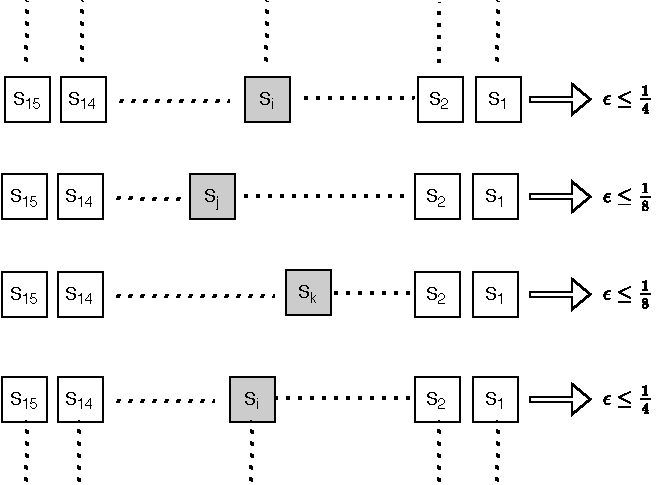
\includegraphics[width=\linewidth]{LC1.pdf}
        \endminipage
        \caption{Bias Calculation}
    \end{figure}
    
\end{frame}

\begin{frame}{Outline of the Proof Cont..}
\begin{itemize}
    \item Bias Calculation : 
    \begin{equation*}
        \epsilon_4^{(4)} \leq 2^{4-1} \times (2^{-2})^2 \times (2^{-3})^2
    \end{equation*}
    \begin{equation*}
        \epsilon_4^{(4)} \leq 2^{-7} 
    \end{equation*}
    \item Case 2 : 5 Active S-boxes involved
    \begin{equation*}
        \epsilon_4^{(5)} \leq 2^{5-1} \times (2^{-2})^4 \times (2^{-3})
    \end{equation*}
    \begin{equation*}
        \epsilon_4^{(5)} \leq 2^{-7} 
    \end{equation*}
    \item Case 3 : More than 5 Active S-boxes involved
    \begin{equation*}
        \epsilon_4^{(i)} \leq 2^{i-1} \times (2^{-2})^i \;\; for \;\; i > 5
    \end{equation*}
    Detailed Proof is given in the report.
\end{itemize}
\end{frame}

\begin{frame}{Requirements for a Successful LC attack}
\begin{itemize}
    \item Maximal Bias of 28-round linear approximation 
    \begin{equation*}
        \epsilon_{28} \leq 2^{6} \times \epsilon_4^{7} = 2^6 \times (2^{-7})^7 \implies \epsilon_{28} \leq 2^{-43}
    \end{equation*}
    \item Assuming the cryptanalyst needs to approximate only 28 Rounds.
    \item Even for single bit key recovery, $N = c|\epsilon|^{-2}$, where constant $c \geq 2$ known plain-texts are required.
    \item Thus, $2^{86}$ known plain-texts are required. 
    \item The data requirement exceeds the total plain-text space available, which is $2^{64}$. 
    \item PRESENT-80 is resistant to Linear attack.
\end{itemize}
    
\end{frame}